\appendix


\section{Requirements}

\subsection{Functional Requirements}

\begin{enumerate}
\item FE integration: System will be able to interface with a third party finite element application

\begin{enumerate}
\item The finite element applications solver must be able to solve a mesh based on its model configuration.
\item The finite element applications solver must be able to execute a model programmatically
\item The finite element applications solver must be able to output stress data at different points on the mesh.
\item The finite element application will provide a graphical representation of the model.
\item It will be possible to manipulate the model that the finite element application uses programmatically.
\item It should be possible to manipulate the model that the finite element application uses from within its graphical user interface.
\end{enumerate}

\item Mesh refinement: System will be able to perform different kinds of finite element mesh refinement

\begin{enumerate}
\item The system will be able to refine a finite element mesh using a stress based refinement method.

\item The system will be able to refine a finite element mesh using a non-stress based refinement method.

\item A non stress based refinement method will adapt the mesh using background information about mesh design which has been previously trained.

\item The system will be able to combine the two methods to produce a coherent mesh which the FE application is able to successfully solve in order to obtain results for stress and displacement.

\item The system will be able to combine both methods to varying degrees that will be performed automatically by the system without direct user intervention.
\item The system will re mesh using both stress and non-stress based refinement using quadrilateral elements.

\item System will adapt weighting associated with each method based upon the metrics computed for the mesh in the systems previous iteration.
\end{enumerate}

\item Quality assessment: System will provide the operator with results about the quality of meshes based on metrics obtained from research.

\begin{enumerate}
\item An assessment will be conducted automatically for every mesh iteration that occurs.

\item System will assess quality based on a variety of metrics to ensure overall robustness of measurement. 

\item The metrics will be computed for both individual element within the model and for the entire mesh.
\end{enumerate}
\end{enumerate}

\newpage
\subsection{Non-Functional Requirements}

\textbf{Design:} The system architecture will be developed using the object oriented design principals of SOLID to allow for clear interfaces between the different functional components. Functional programming practices will be adopted through use of the .NET Language Integrated Query or LINQ framework. This will help to simplify the code and improve reliability by removing unnecessary state from the program. Where functions and classes are written their length will be kept to a minimum to reduce complexity and allow for reuse wherever possible. \\ 

\noindent
\textbf{Documentation:} The system will be comprehensively documented at both a code level and at an architecture level. At a code level C\# doc comments will be written to provide a comprehensive summary of each function. This will allow the tool Doxygen \cite{Doxygen} to generate a full set of developer documentation upon completion of the software implementation which will be included as an appendix. Ensuring that the majority of information is present within doc comments will also help to promote a reduction of loose comments within the code and hence function size. \\

\noindent
\textbf{General applicability:} In order to demonstrate that hybrid methods are a feasible means of approaching meshing problems the resulting software should be able to successfully execute on a range of models with varying geometry. The range of geometries should be representative of typical structural variation encountered by engineers.

\newpage
\section{Element Types within LISA}
Here are shown the the visual specifications LISA provides for the ordering and layout of nodes for defining each type of element supported. Each of these element types can be classified using base classes which implement the IElement interface.

\begin{figure}[!h]
\centering
\begin{subfigure}{.5\textwidth}
  \centering
  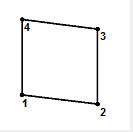
\includegraphics[width=0.3\linewidth]{../Graphics/LISA-quad4.png}
  \caption{quad4 element}
  \label{fig:sub1}
\end{subfigure}%
\begin{subfigure}{.5\textwidth}
  \centering
  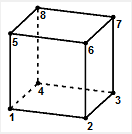
\includegraphics[width=0.3\linewidth]{../Graphics/LISA-hex8.png}
  \caption{hex8 element}
  \label{fig:sub2}
\end{subfigure}
\label{fig:test}
\caption{Square based elements}
\end{figure}


\begin{figure}[!h]
\centering
\begin{subfigure}{.5\textwidth}
  \centering
  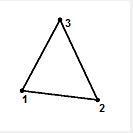
\includegraphics[width=0.3\linewidth]{../Graphics/LISA-tri3.png}
  \caption{tri3 element}
  \label{fig:sub1}
\end{subfigure}%
\begin{subfigure}{.5\textwidth}
  \centering
  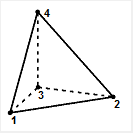
\includegraphics[width=0.3\linewidth]{../Graphics/LISA-tet4.png}
  \caption{tet4 element}
  \label{fig:sub2}
\end{subfigure}
\label{fig:test}
\caption{Triangular based elements}
\end{figure}


\begin{figure}[ht]
\centering
\begin{subfigure}{.5\textwidth}
  \centering
  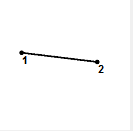
\includegraphics[width=0.3\linewidth]{../Graphics/LISA-line2.png}
  \caption{line2 element}
  \label{fig:sub1}
\end{subfigure}%
\begin{subfigure}{.5\textwidth}
  \centering
  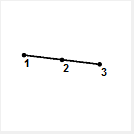
\includegraphics[width=0.3\linewidth]{../Graphics/LISA-line3.png}
  \caption{line3 element}
  \label{fig:sub2}
\end{subfigure}
\label{fig:test}
\caption{Line based elements}
\end{figure} 

%\section{Calculating Centripetal Force For Paper Mill}
%Assuming a constant speed of the paper mill disk at  the following standard calculation was done to compute a forces that could be specified for different elements in order to simulate the effects on the model.

%F = m $\omega^2$ r\\ 

%where: \\ 
%m - mass of object \\ 
%r - radius from centre \\ 
%$\omega$ - angular velocity (radians per second)

%Using the following values for each variable for the plates forming the outside of the paper mill disk the force could be calculated as:

%mass- paper mill is made of steel with each plate having a volume of approximately $24cm^3$ which gives a mass of
%188 grams

\newpage
\section{Unit Testing}
Below can be seen the test explorer interface within Visual studio, tests have also been included in the submission with the rest of the code.

\begin{figure}[H]
  \centerline{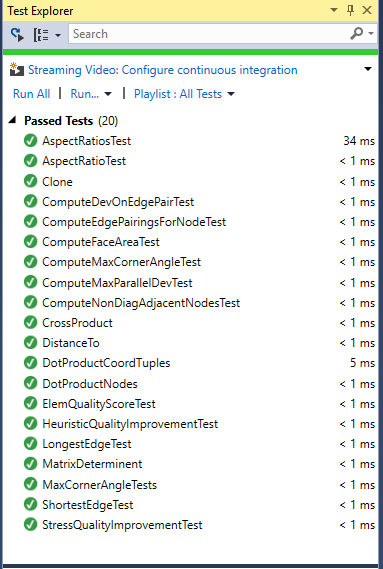
\includegraphics[width=75mm, scale=0.5]{../Graphics/unitTests.png}}
  \caption{Visual Studio window showing the small suite of twenty tests for validating the core functionalyu of the system.}
\end{figure}

%{Centripetal}

\newpage
\section{Edge Definition Categories}
This appendix shows the different values that can be assigned to each of the different edge properties used by the program. Each of these properties has some relevance to the rules and is used to determine how much meshing should occur along a particular edge. \\ 

\textbf{Edge Type}
\begin{itemize}
  \item important long
  \item important
  \item important short
  \item not important
  \item circuit
  \item half circuit
  \item quarter circuit
  \item short for a hole
  \item long for a hole
  \item circuit hole
  \item half circuit hole
  \item quarter circuit hole
\end{itemize}

\textbf{Boundary Type}
\begin{itemize}
  \item free
  \item fixed on one side
  \item fixed on two sides
  \item fixed completely
\end{itemize}

\textbf{Load Type}
\begin{itemize}
  \item no loading
  \item one side loaded
  \item two sides loaded
  \item continuous loading
\end{itemize}

\newpage

\section{Input and Output Files}
Below can be seen the format of the input files for the system, a LISA .liml and a .json edge definition file. Examples of both these files have also been included within the submission under the ``Experiments'' folder. \\

\begin{figure}[H]
  \centerline{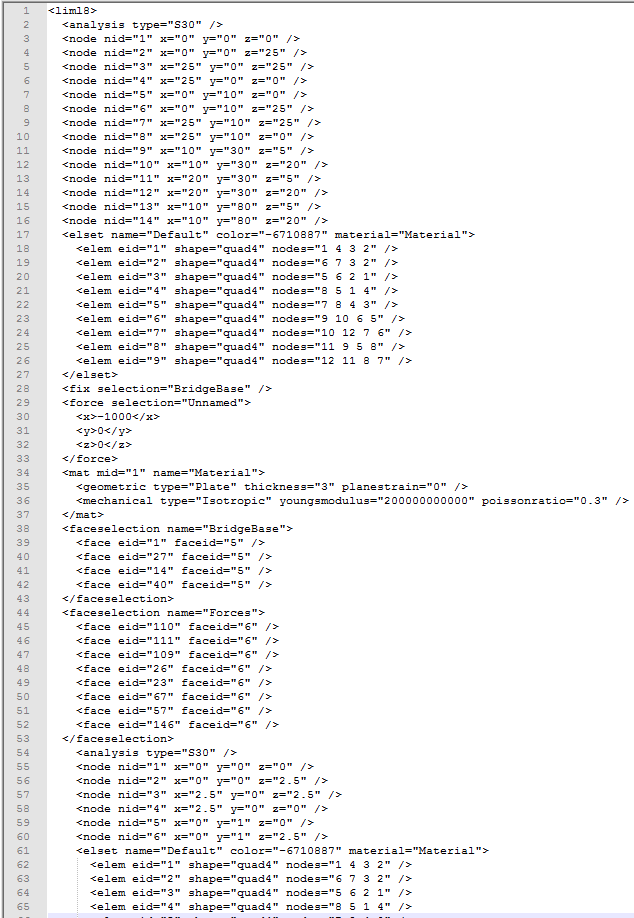
\includegraphics[width=120mm,  scale=0.5]{../Graphics/limlFileLayout.png}}
  \caption{Cut down .liml file to show general content which largely defined the schema for the systems data model}
\end{figure}


\begin{figure}[H]
  \centerline{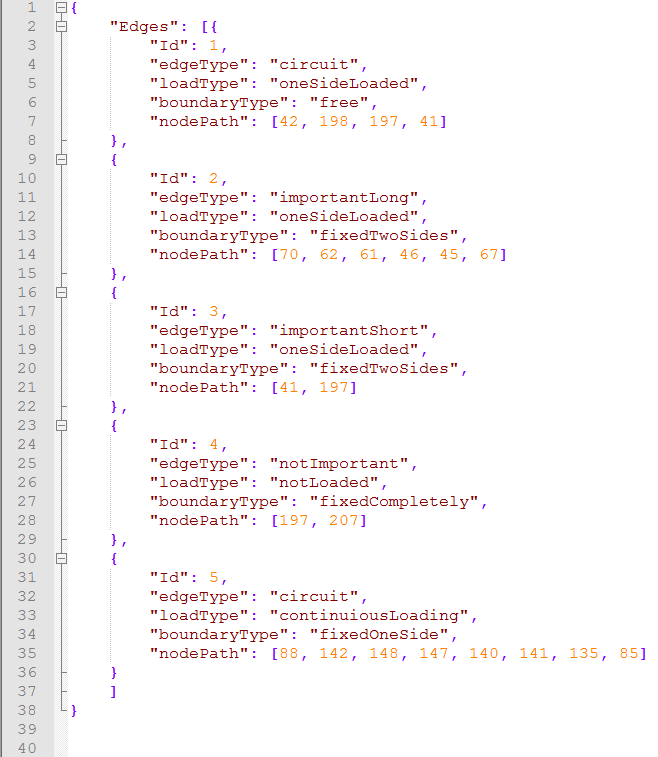
\includegraphics[width=120mm,  scale=0.5]{../Graphics/jsonEdgeFileLayout.png}}
  \caption{A json file containing the edges of interest specified by an engineer, this is parsed and the rules are applied to determine the models meshing based on the input}
\end{figure}


%\begin{subfigure}{.5\textwidth}
%  \centering
%  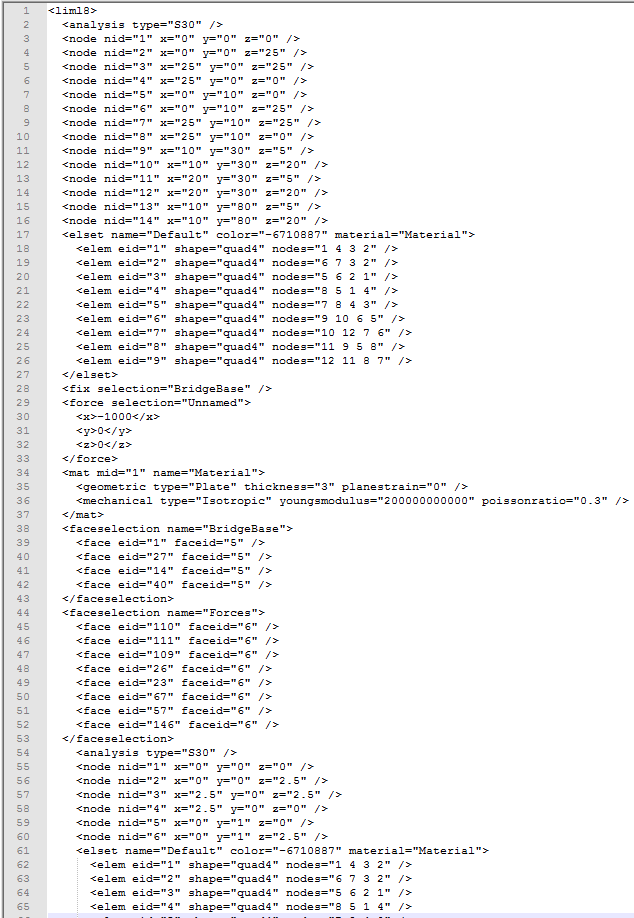
\includegraphics[width=0.6\linewidth]{../Graphics/limlFileLayout.png}
%  \caption{Cut down .liml file to show general content which largely defined the schema for the systems data model}
%  \label{fig:sub1}
%\end{subfigure}%
%\begin{subfigure}{.5\textwidth}
%  \centering
%  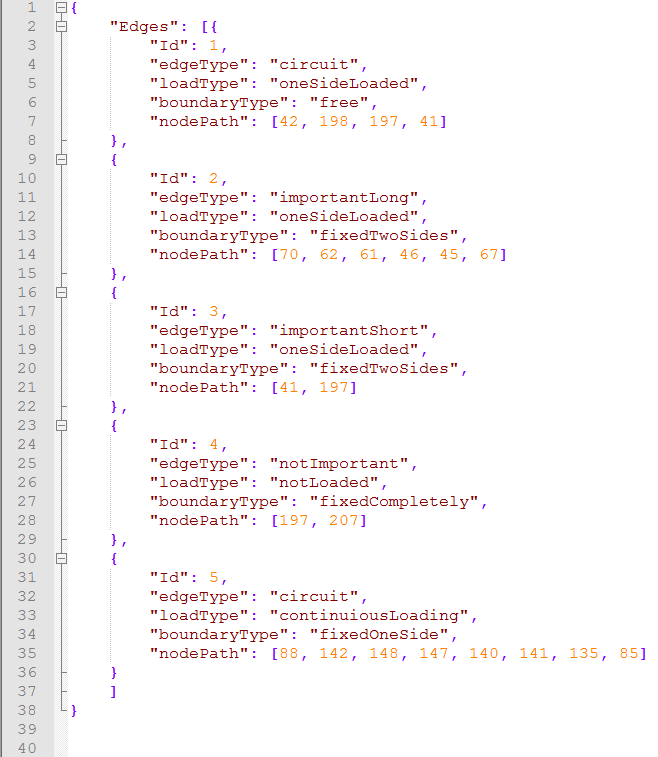
\includegraphics[width=0.8\linewidth]{../Graphics/jsonEdgeFileLayout.png}
%  \caption{A json file containing the edges of interest specified by an engineer, this is parsed and the rules are applied to determine the models meshing based on the input}
%  \label{fig:sub2}
%\end{subfigure}
%\label{fig:test}


\newpage
\section{Project Layout in Solution Explorer}
Below show the Visual Studio Solution Explorer which provides a general idea of the layout of the project with namespace hierarchies from within an IDE.

\begin{figure}[H]
  \centerline{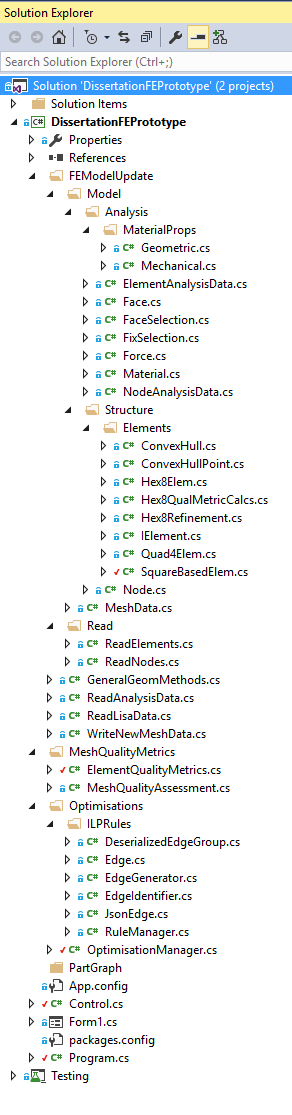
\includegraphics[width=60mm, height=180mm, scale=0.25]{../Graphics/VSolutionExplorer.png}}
  \caption{The metrics calculated by visual studio for all high level modules in the system}
\end{figure}



\newpage
\section{Doxygen Documentation}
Here can be seen two screenshots of the documentation that was automatically generated using the tool , the full documentation has been included as part of the supporting material for the dissertation. 

\begin{figure}[H]
  \centerline{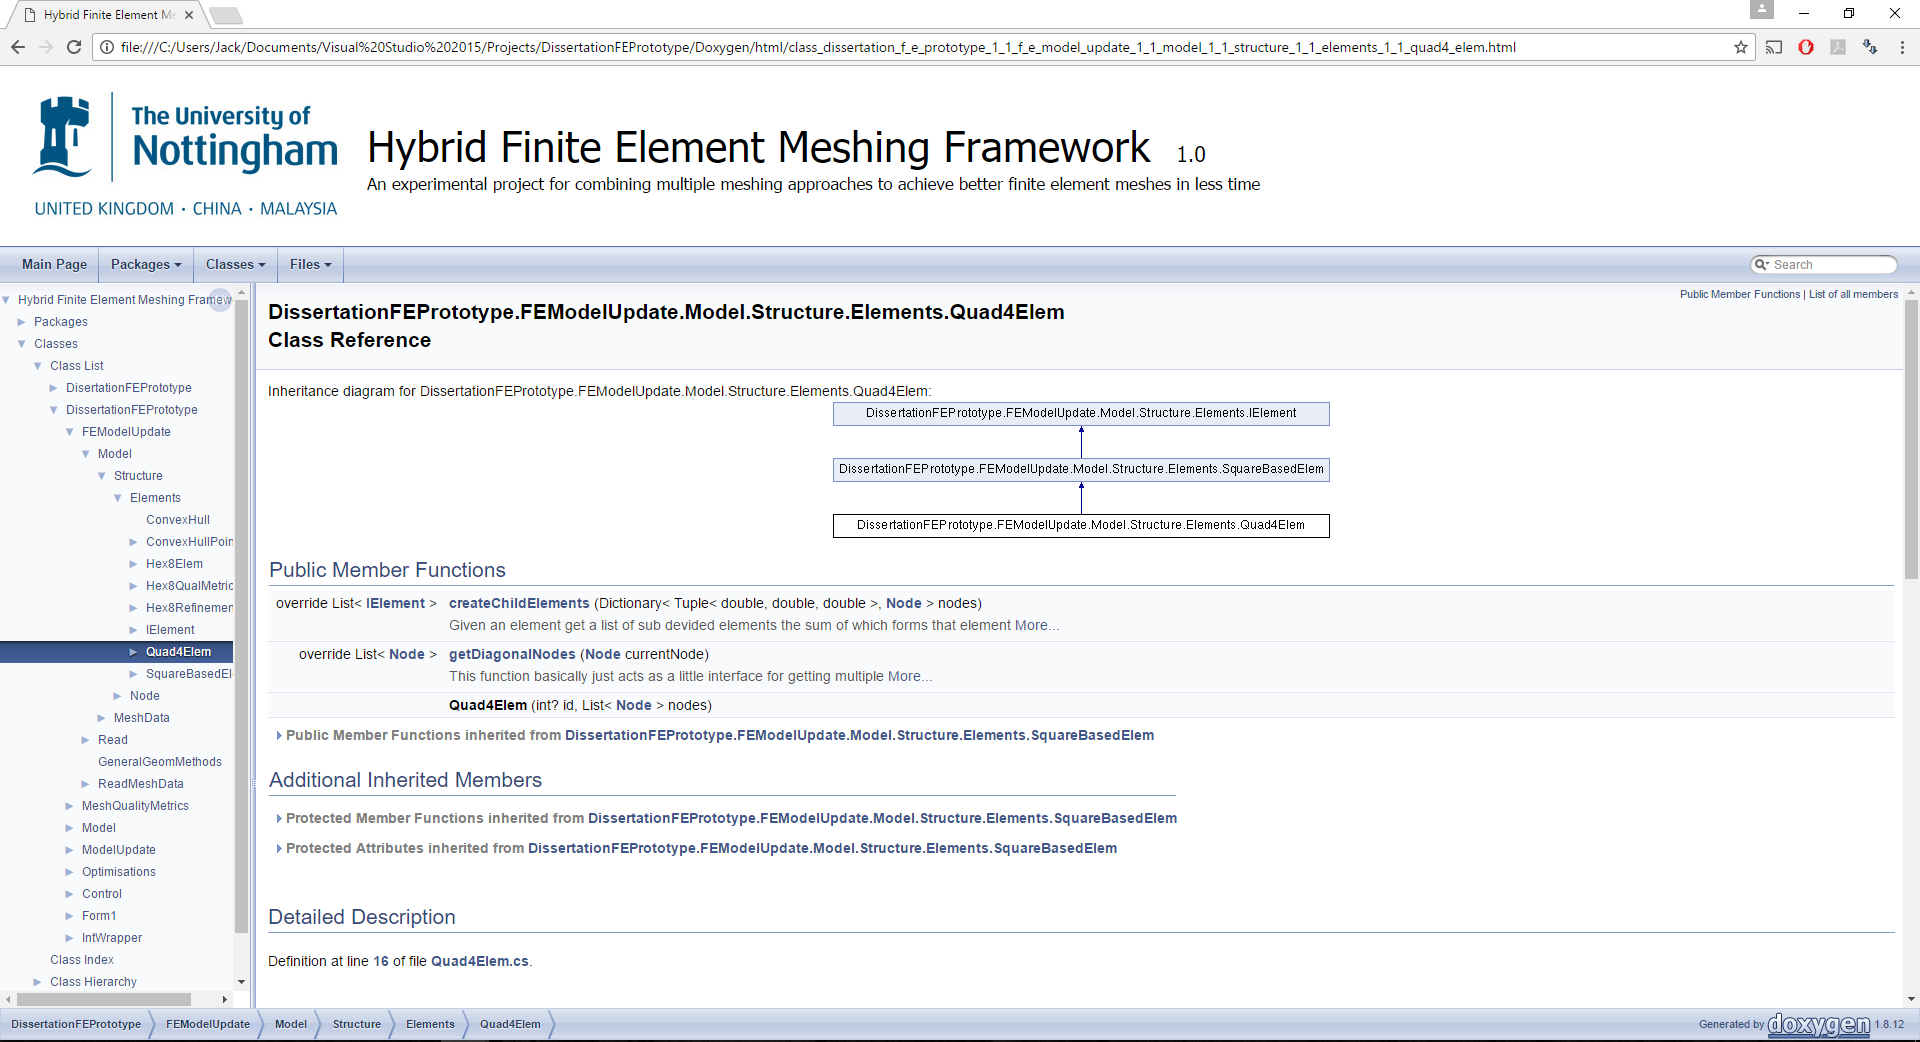
\includegraphics[width=150mm,  scale=0.5]{../Graphics/Doxygen/Quad4Element.png}}
  \caption{The manual page for the Quad4 element class with the class hierarchy and specific public methods}
\end{figure}

\begin{figure}[H]
  \centerline{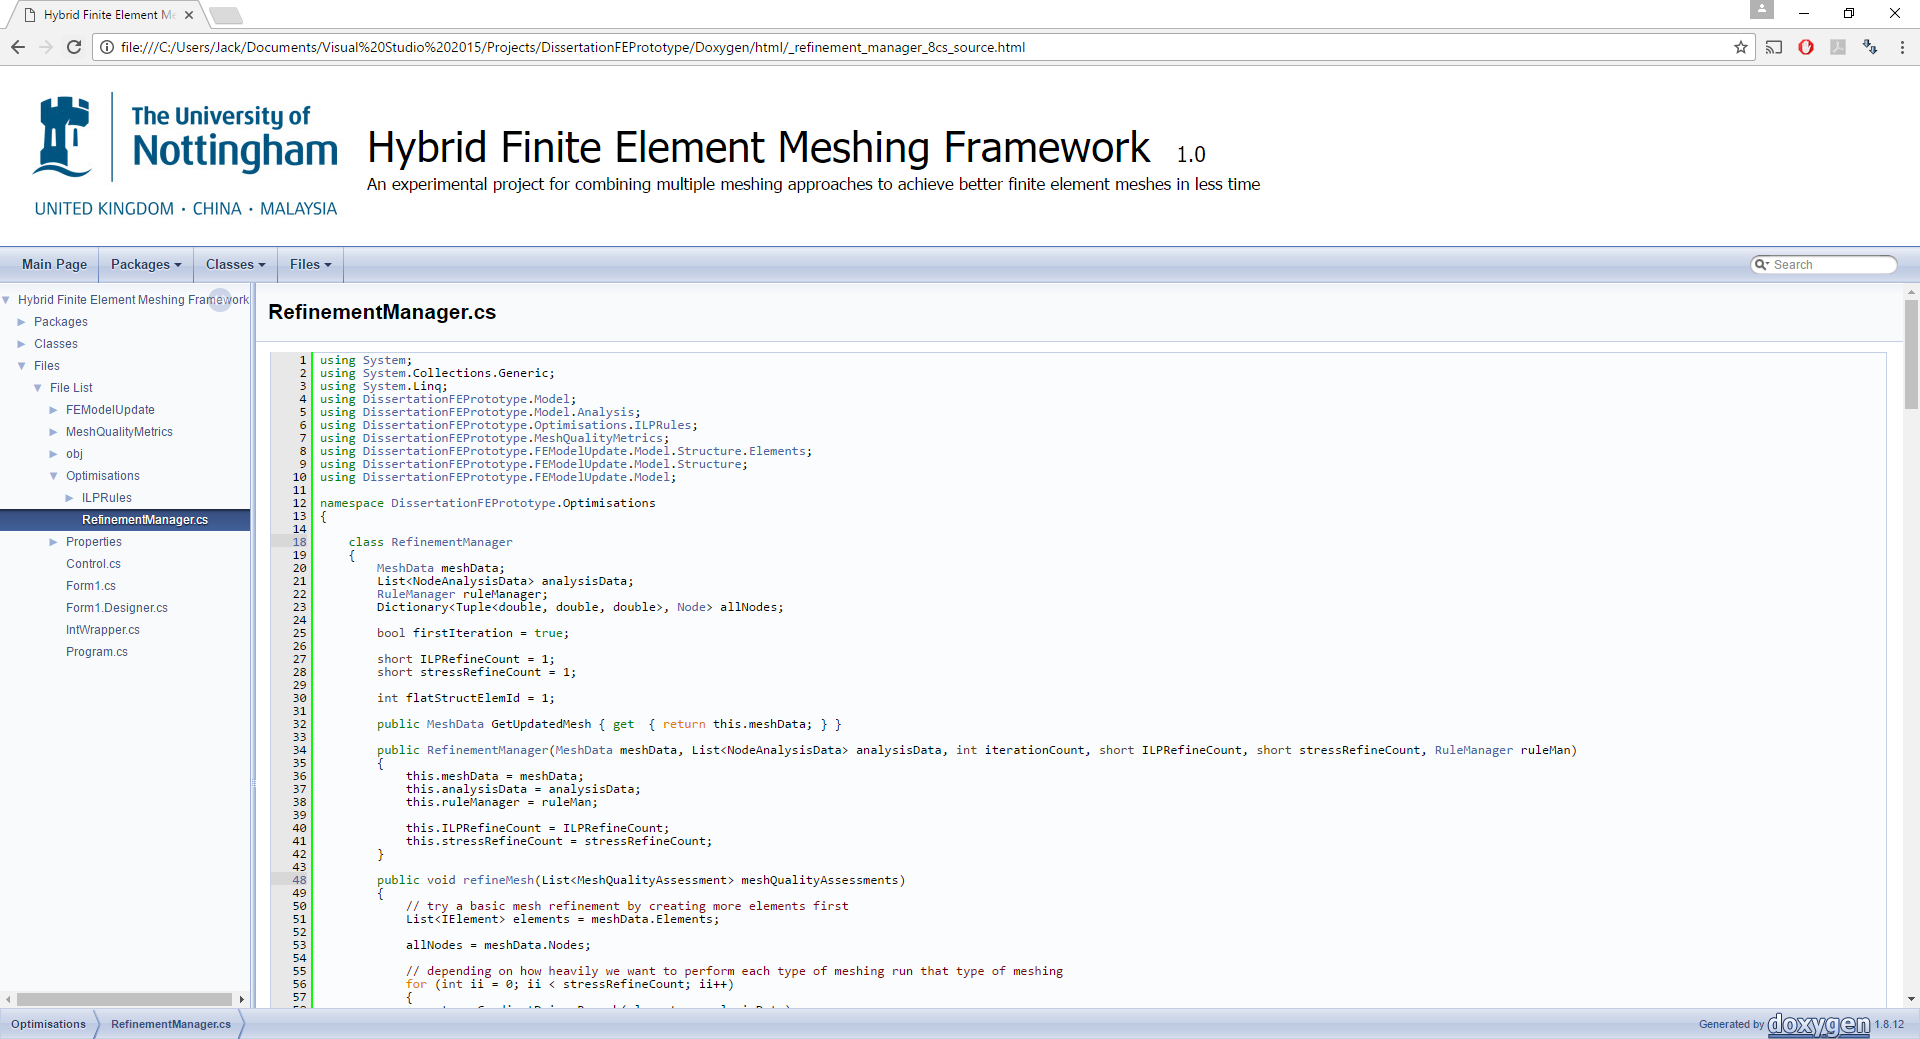
\includegraphics[width=150mm,  scale=0.5]{../Graphics/Doxygen/RefinementManager.png}}
  \caption{Code for the RefinementManager class viewed within the Doxygen UI}
\end{figure}


\newpage
\section{Software Quality Metrics}
This appendix shows some of the code metric results calculated by visual studio for the final software implementation.
\begin{figure}[H]
  \centerline{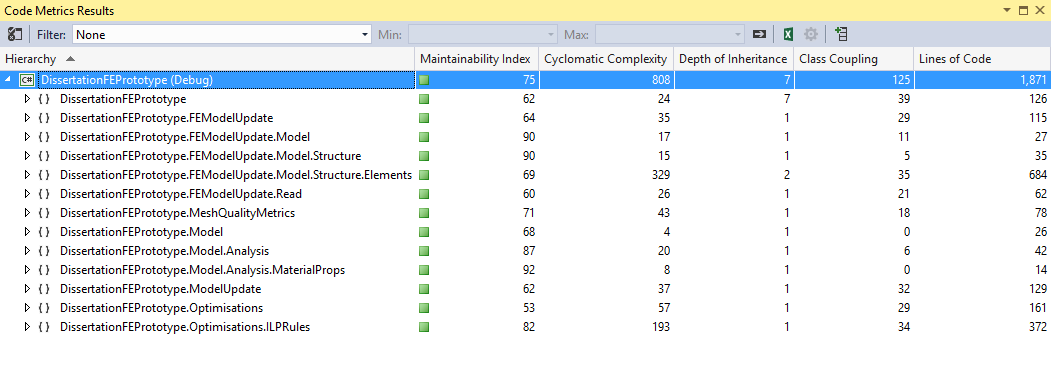
\includegraphics[width=165mm, scale=0.5]{../Graphics/softwareQualityMetrics.png}}
  \caption{The metrics calculated by visual studio for all high level modules in the system}
\end{figure}

\begin{figure}[H]
  \centerline{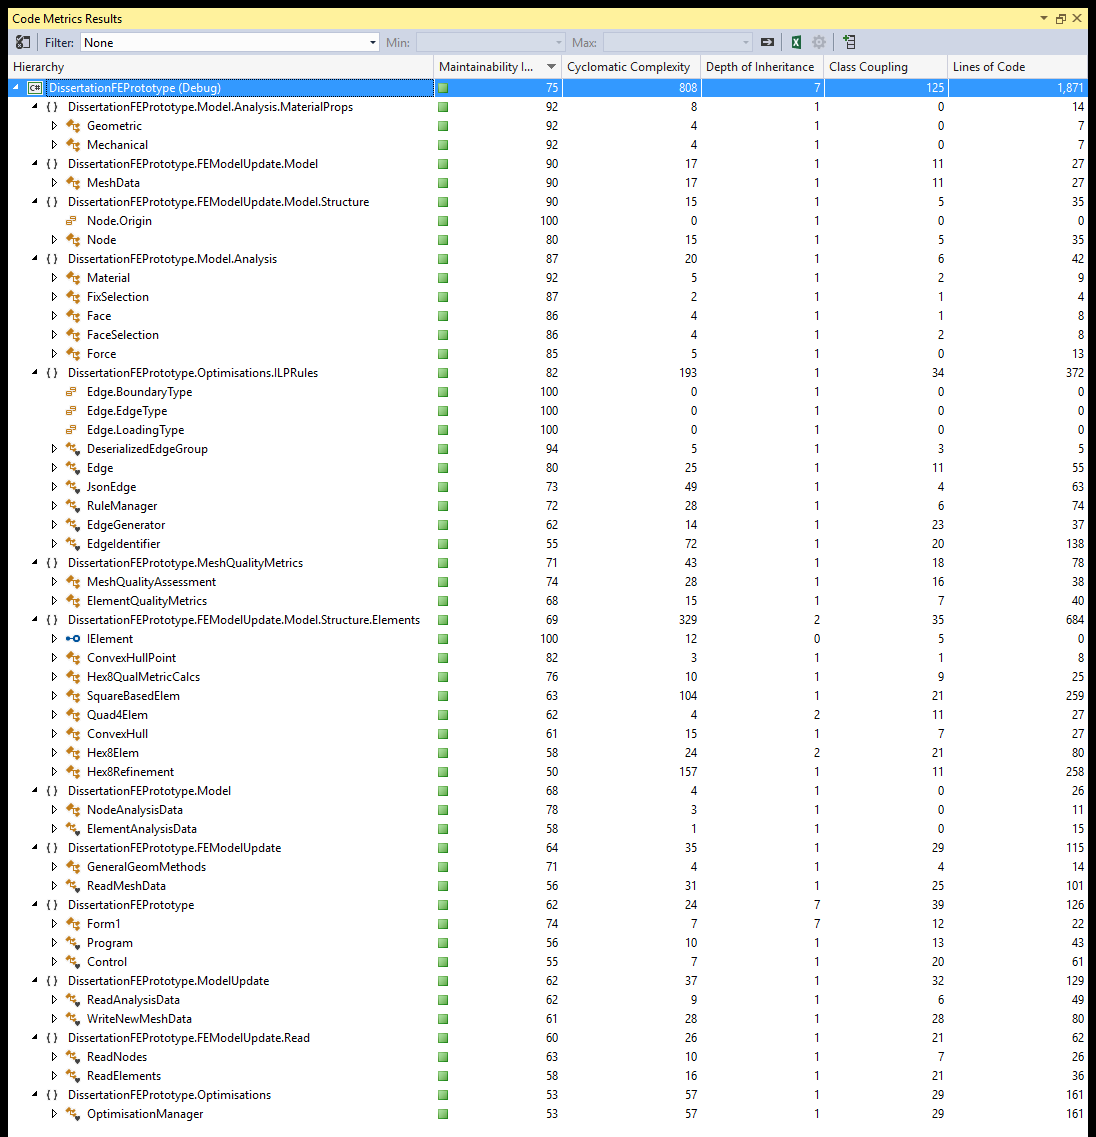
\includegraphics[width=165mm, scale=0.5]{../Graphics/qualityMetricsExpanded.png}}
  \caption{The metrics calculated by visual studio for the all classes in the final system}
\end{figure}

\newpage
\section{Sorting Nodes by Splitting With Planes}
\noindent
Attempting to arrive at a more general solution for sorting nodes in 3D space focus was directed towards the more complex Hex8 element type as this represented a more complete example of a node sorting problem that may have to be solved. Consideration of Hex8 elements led to the realisation that the most important task in sorting nodes for an arbitrary type is to simply establish the corner nodes relative to that type. Having established corners correctly sorting then simply required adding them to a list in the order specified by LISA. \\

\noindent
The subsequent method which was used to successfully establish corners for both Quad4 and Hex8 elements during the earlier prototyping stages of the project was to split nodes for each element using planes running along the x, y and z axis as can be seen in Figure 9 below.

\begin{figure}[!h]
\centering
\begin{subfigure}{.5\textwidth}
  \centering
  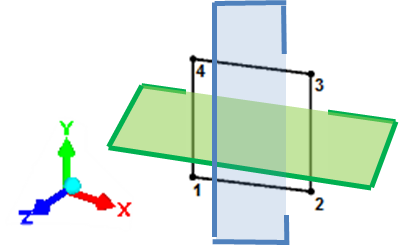
\includegraphics[width=0.9\linewidth]{../Graphics/SortingQuad4.png}
  \caption{Dividing a Quad4 along planes to establish each node as a corner point}
  \label{fig:sub1}
\end{subfigure}%
\begin{subfigure}{.5\textwidth}
  \centering
  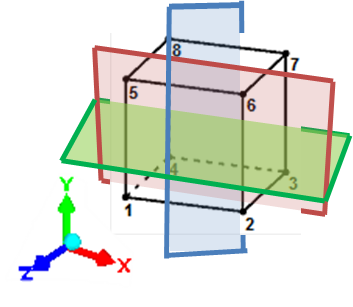
\includegraphics[width=0.7\linewidth]{../Graphics/SortingHex8.png}
  \caption{Dividing a Hex8 along planes to establish each node as a corner point}
  \label{fig:sub2}
\end{subfigure}
\caption{Splitting Element points using x, y and z planes in order to perform ordering for LISA}
\label{fig:test}
\end{figure}

\noindent
Although this approach resolved the initial problems resulting from simply trying to traverse the nodes it did not offer a strong general case solution to the problem with the code for a Hex8 element needing to be significantly different and more complex than that of a Quad4 and with the potential for the most complex FE element types such as wedge15, hex20, and pyr13 there would again be an even greater numbers of plane divisions yet again.

\newpage
\section{Mesh Refinements}
This appendix item attempt too show the general mesh that are formed using the heuristic and stress based refinement strategy with examples of where a heuristic has been placed well and poorly and where there is also variation in the threshold used to decide whether elements are meshed with the stress variable. Although in the rest of the models we are looking for stress since this is the primary variable of interest displacement has been selected as the analysis variable for displacement due to it producing a clearer gradient than stress.

\subsection{Heuristic Refinement}
\begin{figure}[H]
\centering
\begin{subfigure}{.5\textwidth}
  \centering
	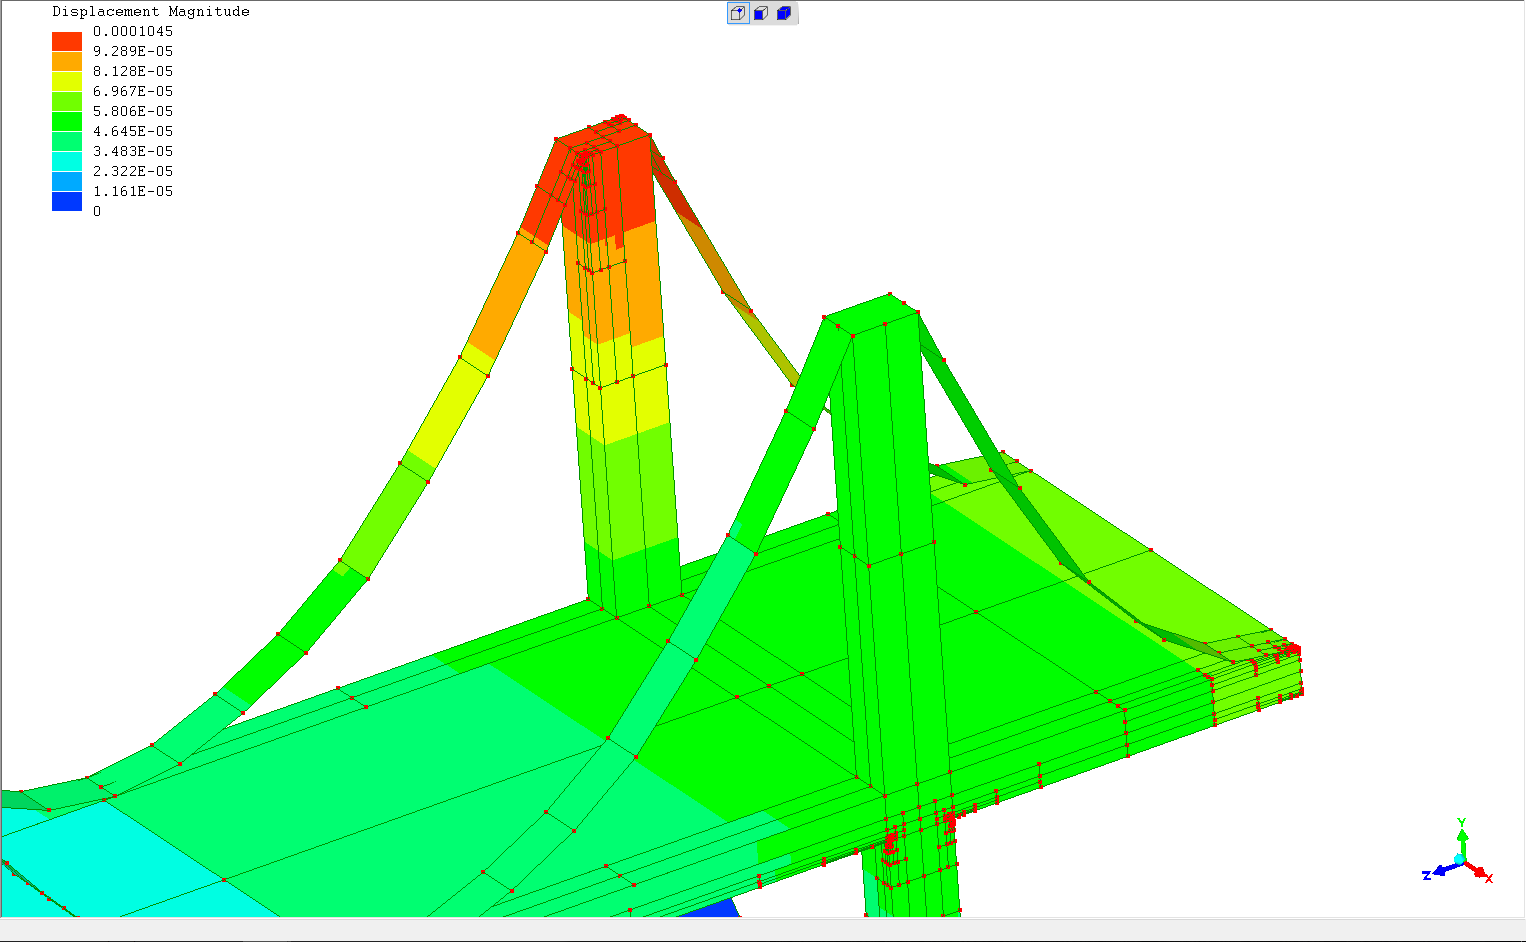
\includegraphics[width=80mm, scale=0.5]{../Graphics/BridgeCrossLoading/bestEdgeSpecResults.png}
  \caption{Important edges specified effectively to facilitate preemptive meshing of area which undergoes high stress}
  \label{fig:sub1}
\end{subfigure}%
\begin{subfigure}{.5\textwidth}
  \centering
  \centerline{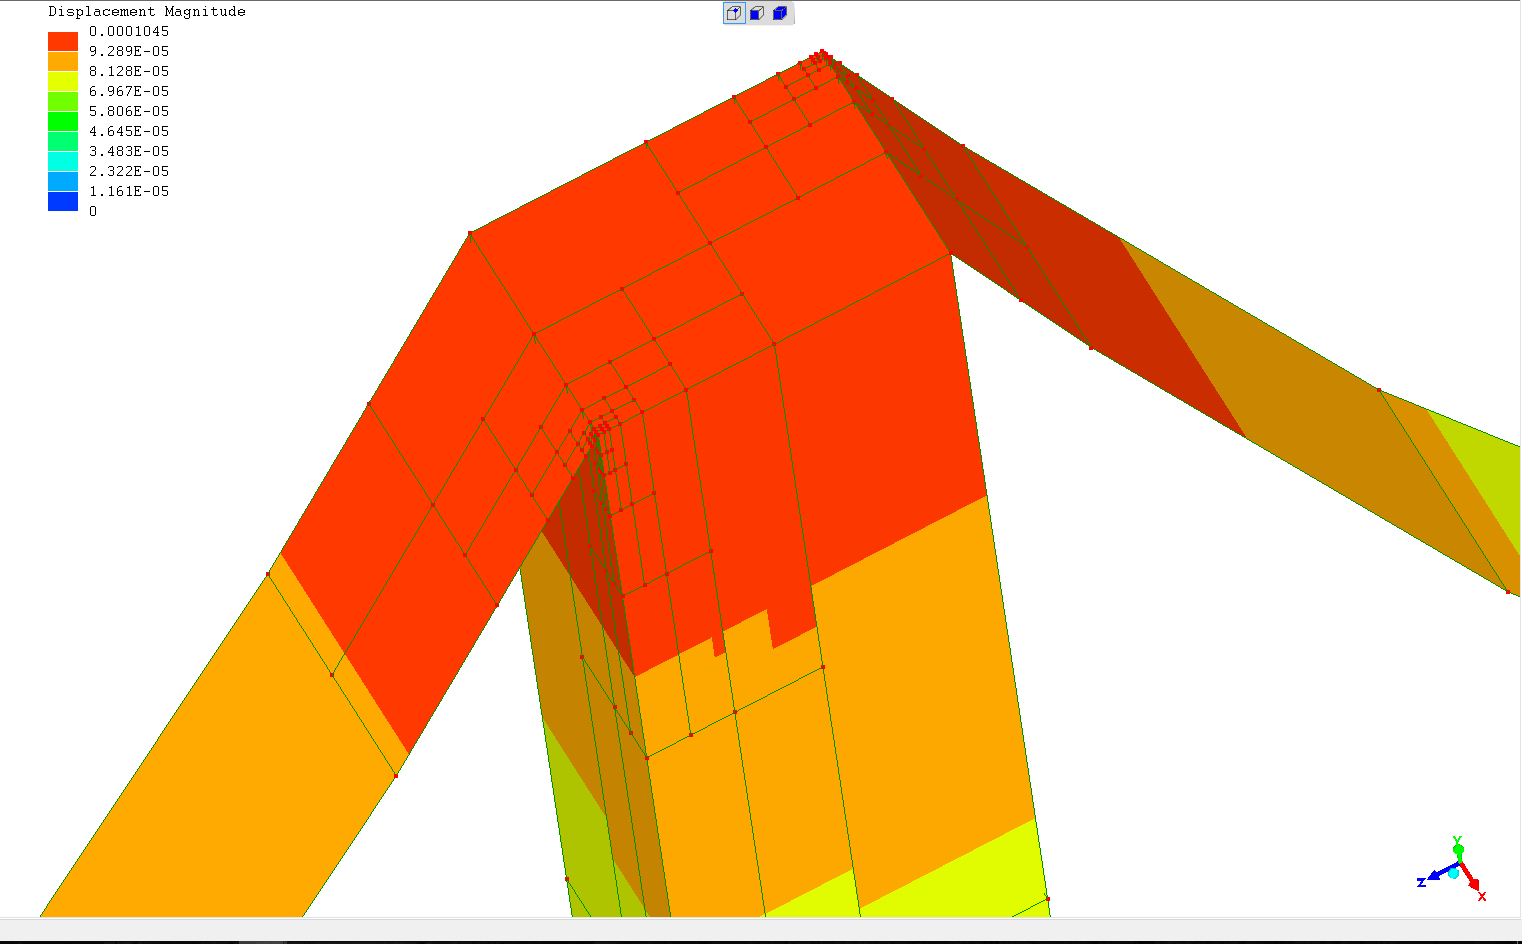
\includegraphics[width=80mm, scale=0.5]{../Graphics/BridgeCrossLoading/bestEdgeSpecResultsCloseUp.png}}
  \caption{Close up view of refinement for high displacement areas }
  \label{fig:sub2}
\end{subfigure}
\label{fig:test}
\end{figure}


\begin{figure}[H]
  \centerline{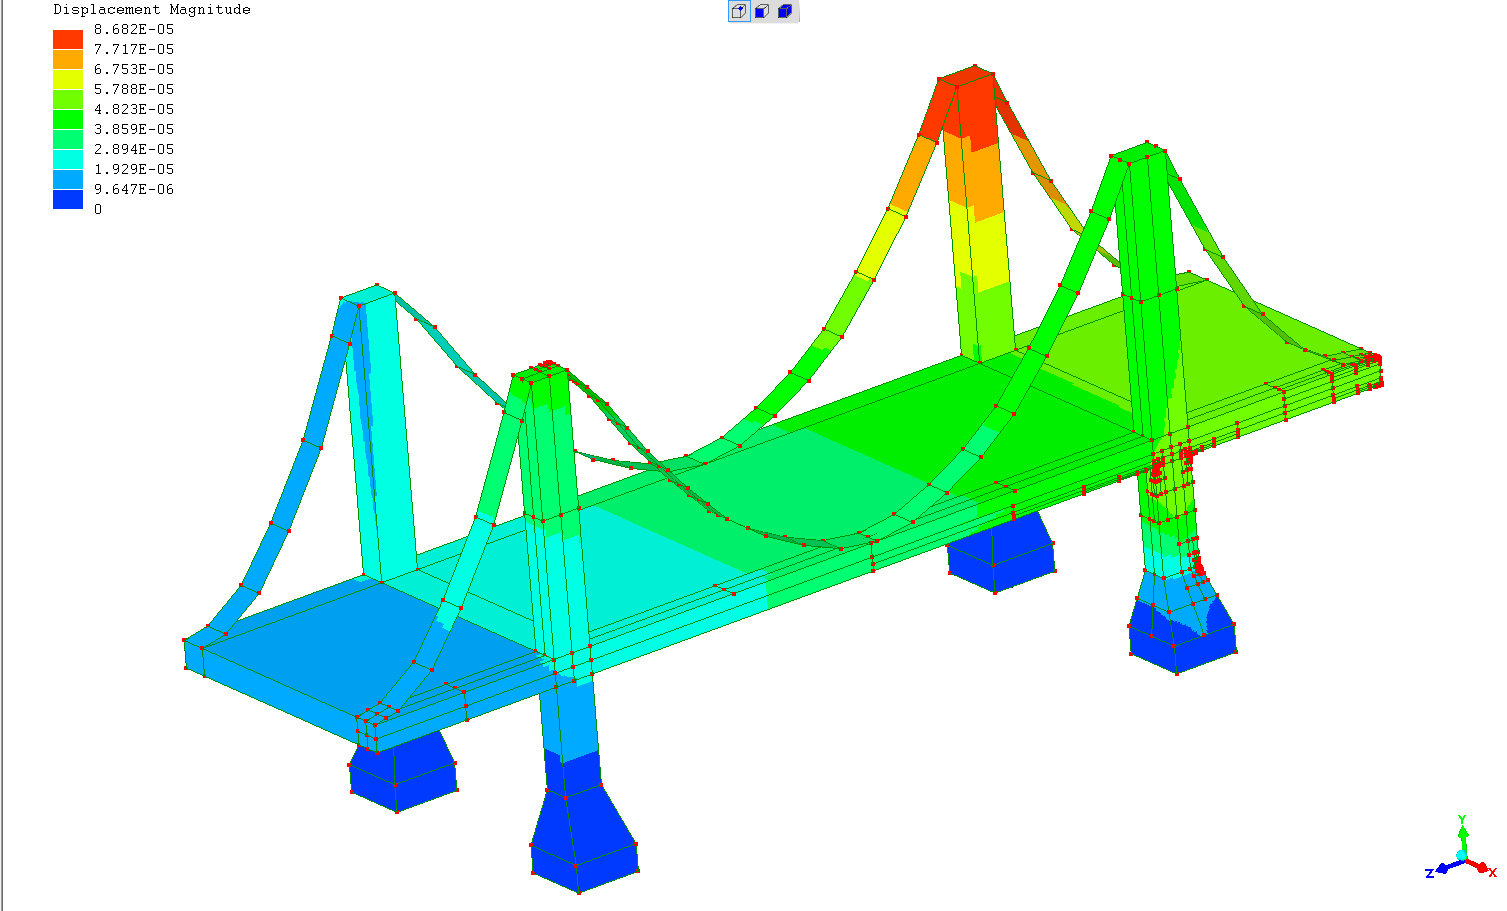
\includegraphics[width=165mm, scale=0.5]{../Graphics/BridgeCrossLoading/okEdgeSpecResults.png}}
  \caption{Important edges more poorly specified missing high displacement region on top of furthest suspension bridge tower}
\end{figure}

\subsection{Stress Refinement}
\begin{figure}[H]
  \centerline{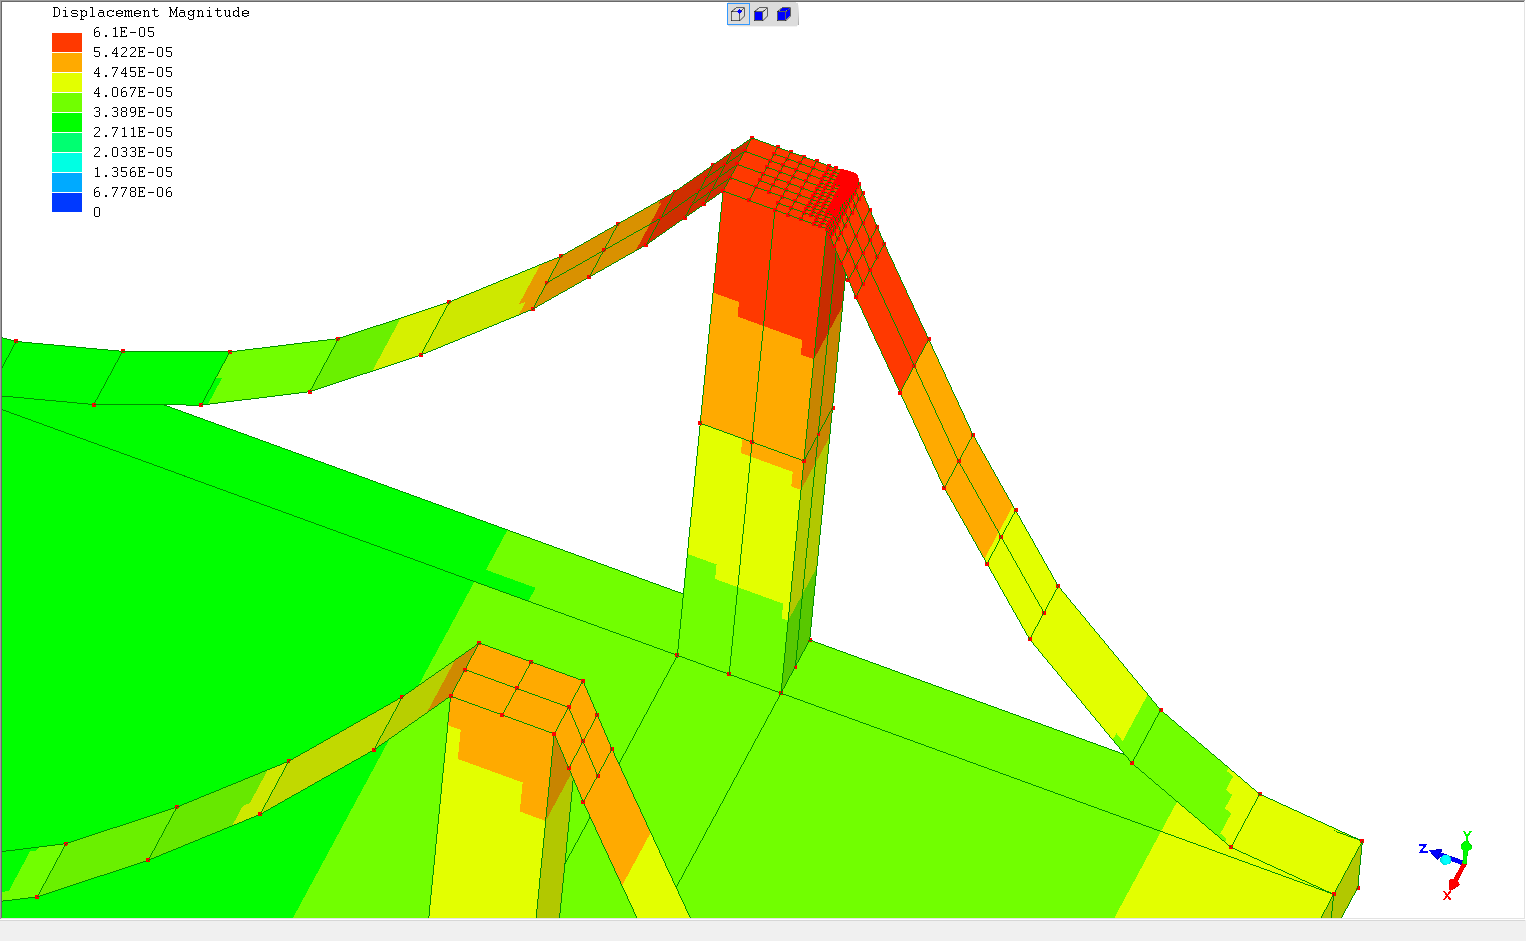
\includegraphics[width=165mm, scale=0.5]{../Graphics/BridgeCrossLoading/the90thPercentileRefinement.png}}
  \caption{Iterative stress/ displacement refinement method used to focus meshing on the top 6\% most displaced region of model}
\end{figure}

\begin{figure}[H]
  \centerline{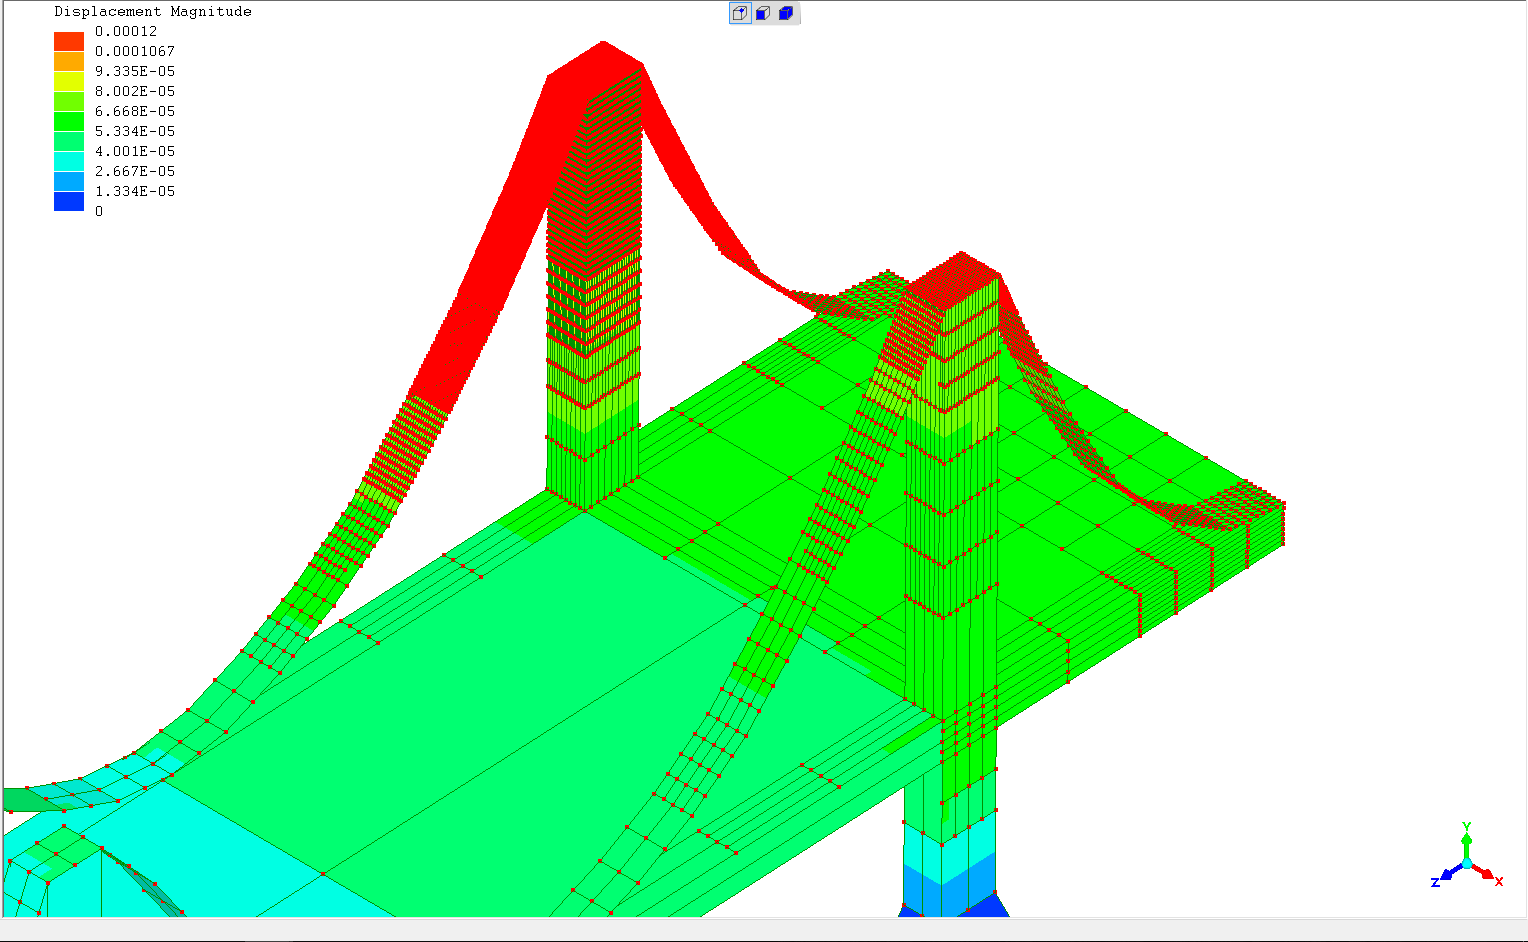
\includegraphics[width=165mm, scale=0.5]{../Graphics/BridgeCrossLoading/aboveAverageRefinement2.png}}
  \caption{Iterative refinement of high displacement but with the remesh threshold specified as the average displacement across the whole model. A consequence of this is the gradient of refinement fidelity that can be seen corresponding to the importance of that part of the structure}
\end{figure}


\begin{figure}[H]
  \centerline{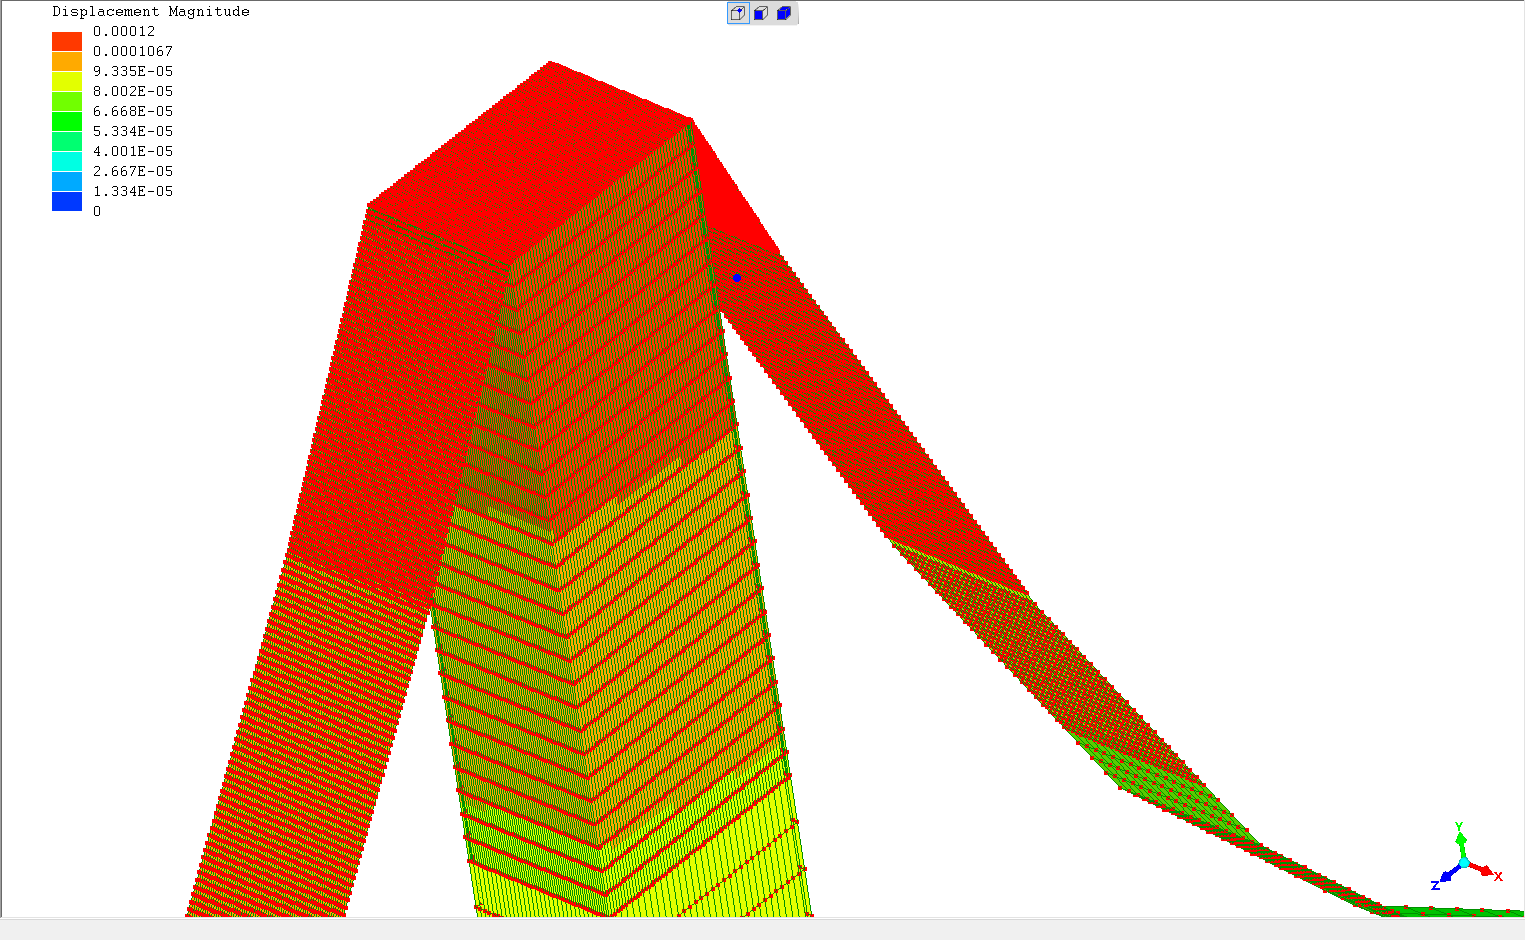
\includegraphics[width=165mm, scale=0.5]{../Graphics/BridgeCrossLoading/aboveAverageRefinement.png}}
  \caption{Closer view of very high meshing intensity}
\end{figure}
%\end{changemargin}

\newpage
\section{Paper Mill Simulation Results}
For the paper mill simulation angular forces were set up around the outside of the disk so as to simulate the effect of the disk rotating at high speed, with it also being pulled outwards in the axial direction. This generated some interesting patches of stress across the main body of the structure which could easily be specified as edge rules. Looking at figure 34 it is possible to see very high range of stress values for stress observable within the model as a consequence of stress concentrating at particular points.

% edge assignement drawign her

\begin{figure}[H]
\centering
\begin{subfigure}{.5\textwidth}
  \centering
  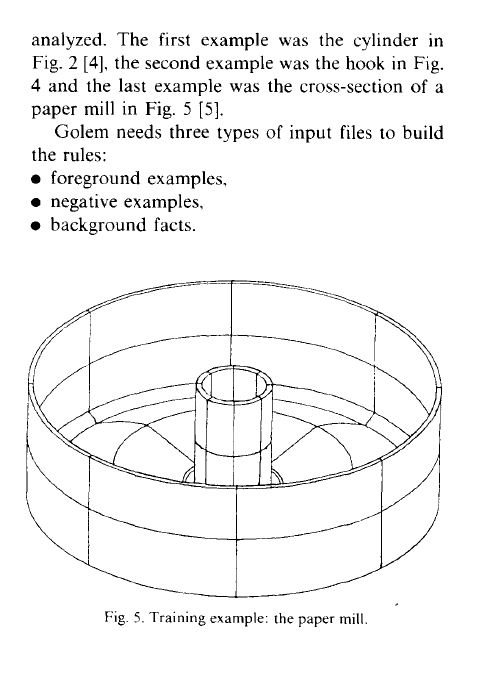
\includegraphics[width=0.9\linewidth]{../Graphics/PaperMillDolsak.jpeg}
  \caption{Half of Cylinder structure described by dolsak in his papers for training ILP system}
  \label{fig:sub1}
\end{subfigure}%
\begin{subfigure}{.5\textwidth}
  \centering
  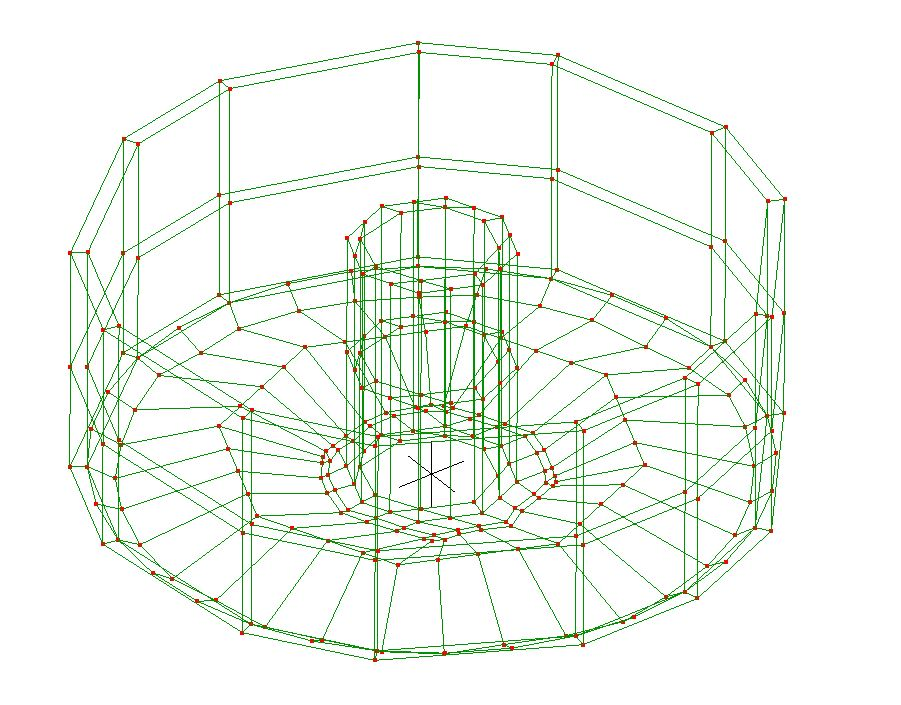
\includegraphics[width=0.9\linewidth]{../Graphics/PaperMillWithinLisa.jpeg}
  \caption{Replication of mesh structure specified by Dolsak within his paper \cite{DolsakPaper91}}
  \label{fig:sub2}
\end{subfigure}
\label{fig:test}
  \caption{Execution time increase compared to the amount of information revealed for the different approaches}
 \end{figure}
 
 \begin{figure}[H]
  \centerline{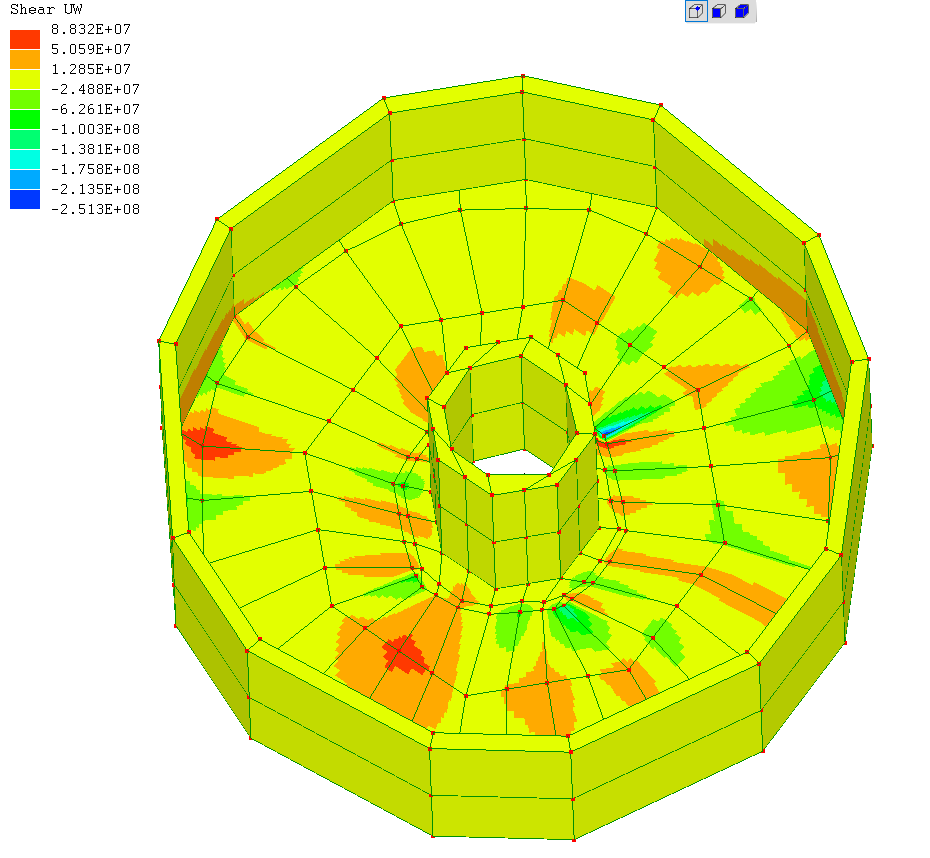
\includegraphics[width=120mm, scale=0.5]{../Graphics/PaperMillStress/PaperMillFirstUWMesh.png}}
  \caption{The initially stressed paper mill part used to define edge sets for further meshing, stress concentrations can be observed in red with colour coding at the top indicating showing a rapidly exponential increase concentrated at those points}
\end{figure}


\begin{figure}[H]
  \centerline{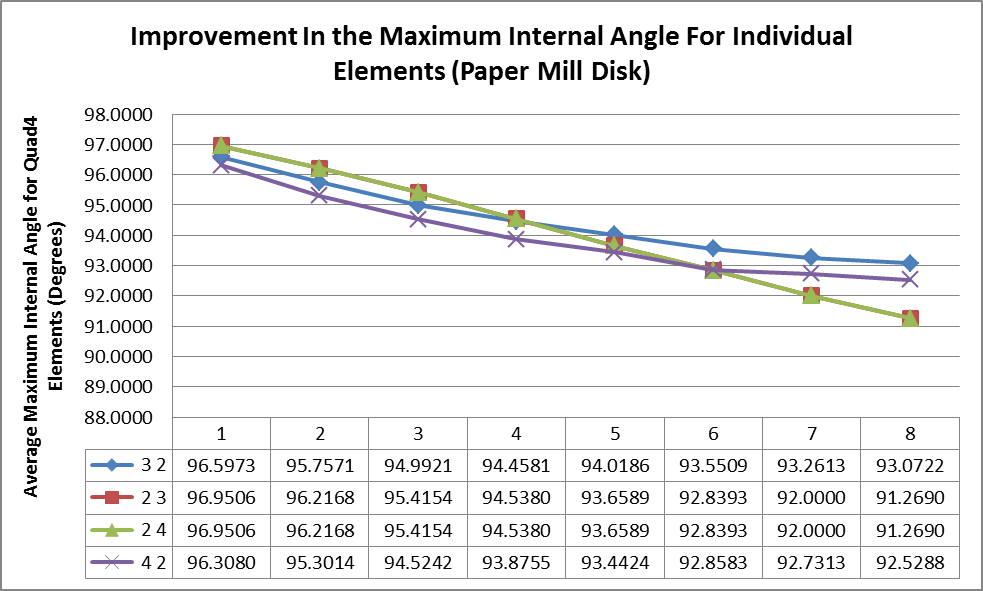
\includegraphics[width=120mm, scale=0.5]{../Graphics/PaperMill/MaximumInternalAngle.png}}
  \caption{Improvement in the maximum internal Angle for Quad4 Elements}
\end{figure}


\begin{figure}[H]
  \centerline{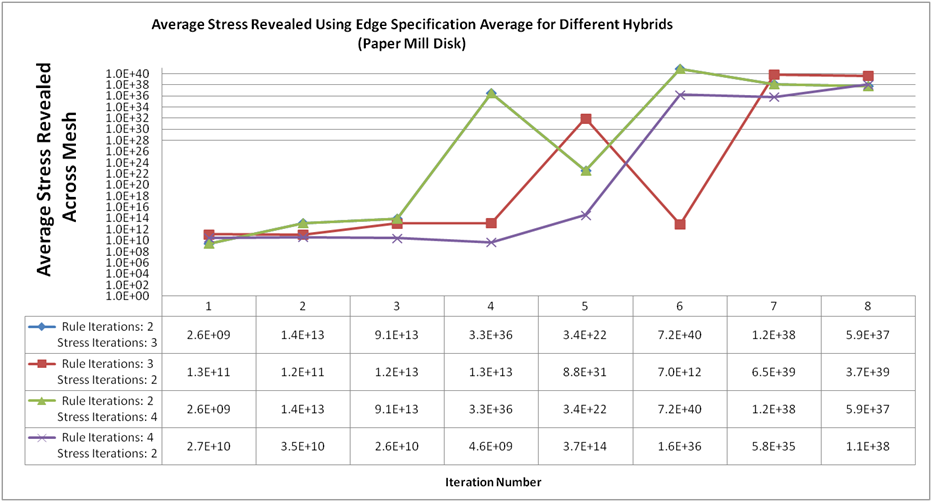
\includegraphics[width=120mm, scale=0.5]{../Graphics/FinalReportGraphs/AverageStressRevealedPaperMill.png}}
  \caption{Improvement on average for detecting across all nodes within the model over multiple iterations, results for each weighting with different edge heuristics also averaged}
\end{figure}



\begin{figure}[H]
  \centerline{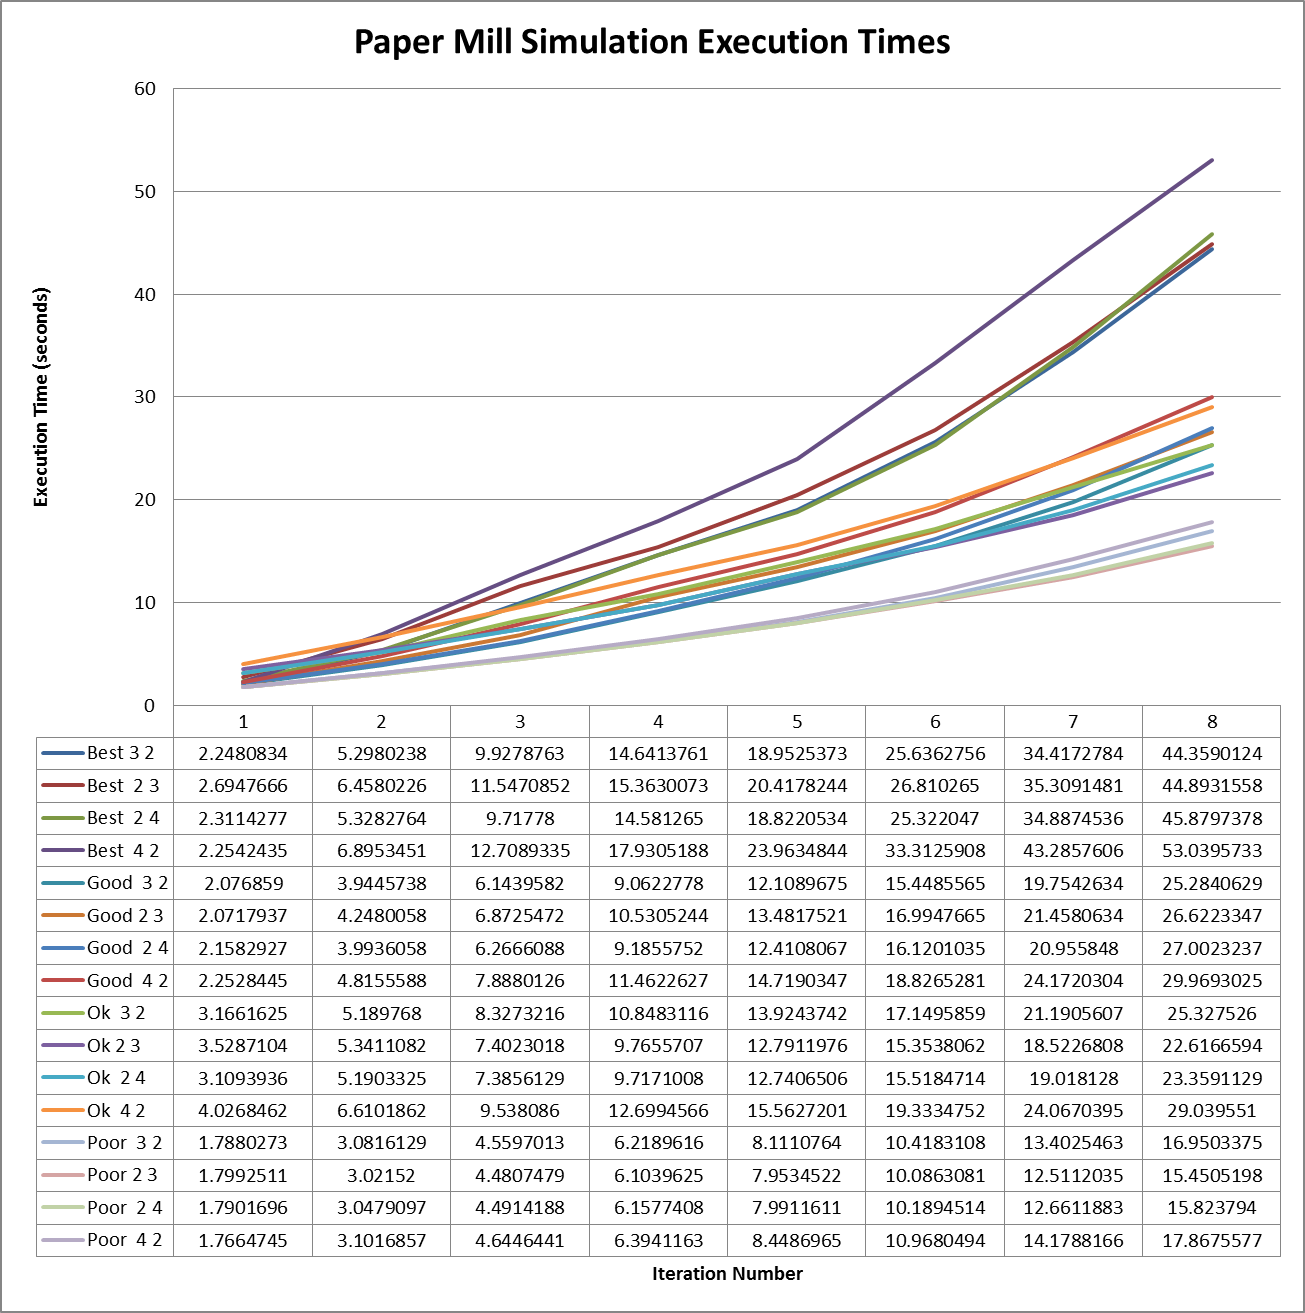
\includegraphics[width=120mm, scale=0.5]{../Graphics/PaperMill/PaperMillExecutionTimes.png}}
  \caption{Time taken per iteration using the different hybrid weightings with varying edge quality specifications}
\end{figure}


\newpage
\section{Half Cylinder Simulation Results}
The half cylinder was the third model used to test the system. 
\begin{figure}[H]
\centering
\begin{subfigure}{.5\textwidth}
  \centering
  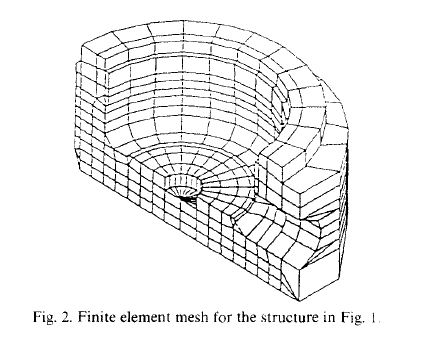
\includegraphics[width=0.9\linewidth]{../Graphics/HalfCylinder/DolsakCylinderMeshed.jpeg}
  \caption{Half of Cylinder structure described by dolsak in his papers for training ILP system}
  \label{fig:sub1}
\end{subfigure}%
\begin{subfigure}{.5\textwidth}
  \centering
  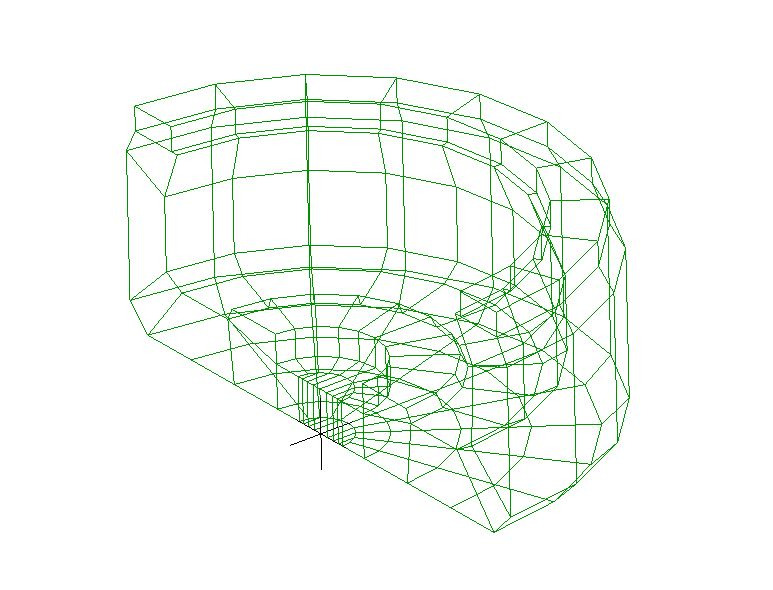
\includegraphics[width=0.9\linewidth]{../Graphics/HalfCylinder/DolsakCylinderWithinLisa.jpeg}
  \caption{Replication of mesh structure specified by Dolsak within his paper \cite{DolsakPaper91}}
  \label{fig:sub2}
\end{subfigure}
\label{fig:test}
  \caption{Execution time increase compared to the amount of information revealed for the different approaches}
 \end{figure}
 
 \begin{figure}[H]
\centering
\begin{subfigure}{.5\textwidth}
  \centering
  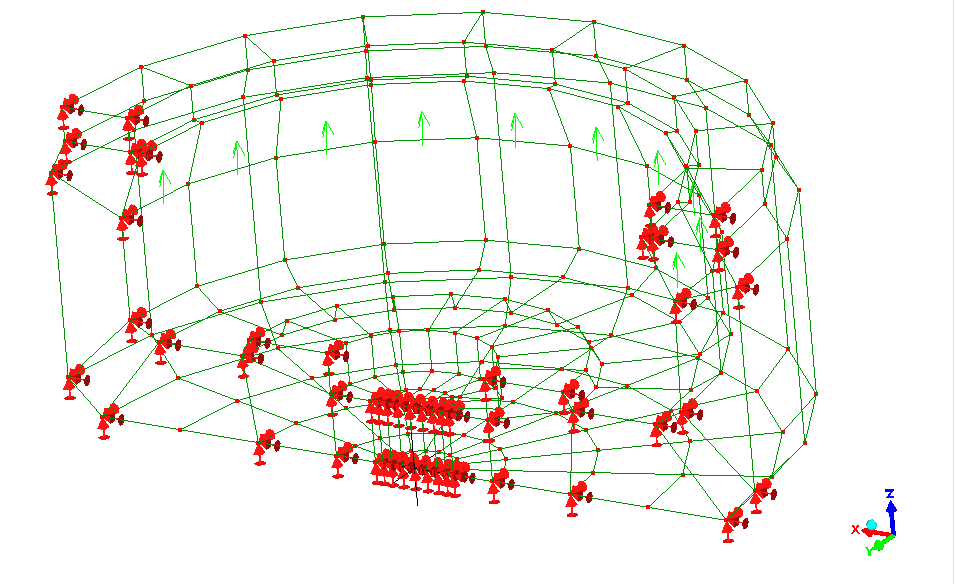
\includegraphics[width=0.9\linewidth]{../Graphics/HalfCylinder/ForcesAndConstraintsOnCylinderPNG.png}
  \caption{Cylinder Constrained by its adjacent half with forces applied up and outwards on its inner rim}
  \label{fig:sub1}
\end{subfigure}%
\begin{subfigure}{.5\textwidth}
  \centering
  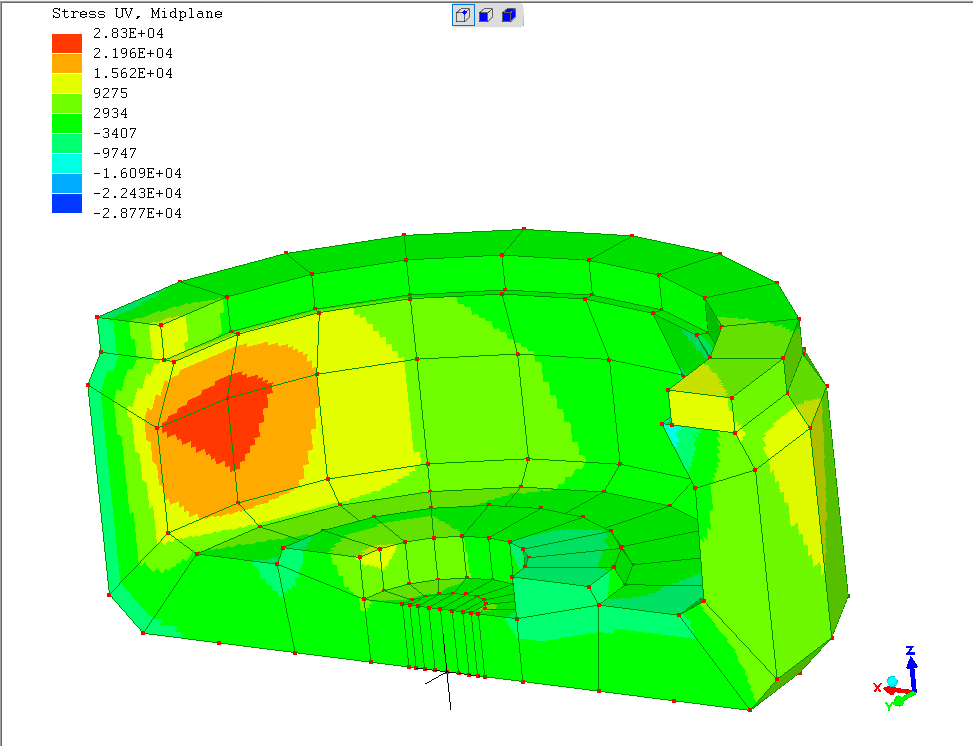
\includegraphics[width=0.9\linewidth]{../Graphics/HalfCylinder/InitialStress.png}
  \caption{Half cylinder with an initial stress concentration having performed a simple execution of the model.}
  \label{fig:sub2}
\end{subfigure}
\label{fig:test}
  \caption{Initial configuration for the half cylinder and some stresses revealed on the structure}
 \end{figure}
 
\begin{figure}[H]
  \centerline{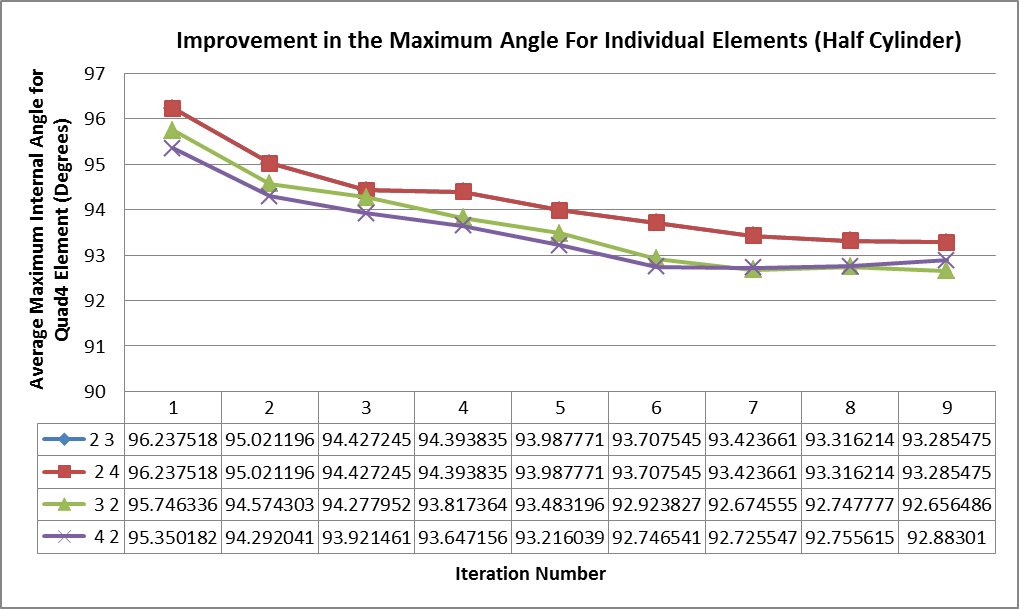
\includegraphics[width=120mm, scale=0.5]{../Graphics/HalfCylinder/ImprovementInMaxCornerAngles.png}}
  \caption{Improvement in corner angles for Quad4 elements using the different hybrid methods on the cylinder}
\end{figure}

\begin{figure}[H]
  \centerline{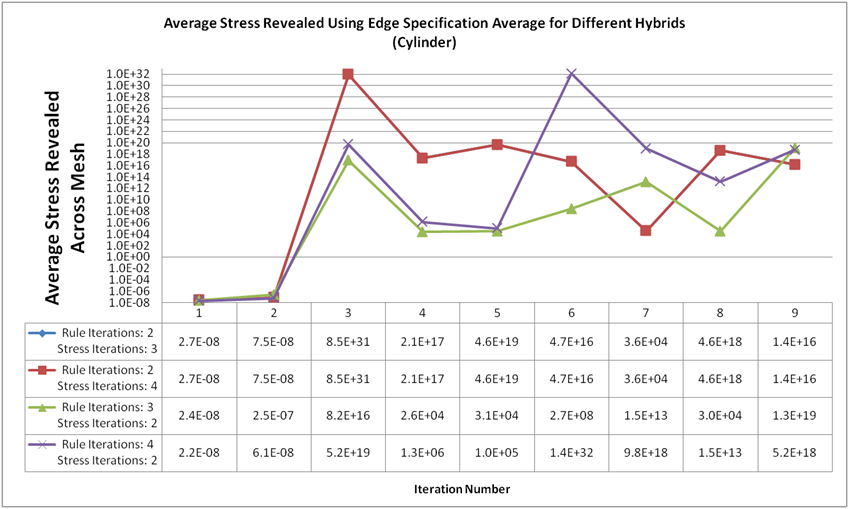
\includegraphics[width=120mm, scale=0.5]{../Graphics/FinalReportGraphs/AverageStressRevealedCylinder.png}}
  \caption{Stress revealed for each iteration using the different hybrid methods}
\end{figure}

\begin{figure}[H]
  \centerline{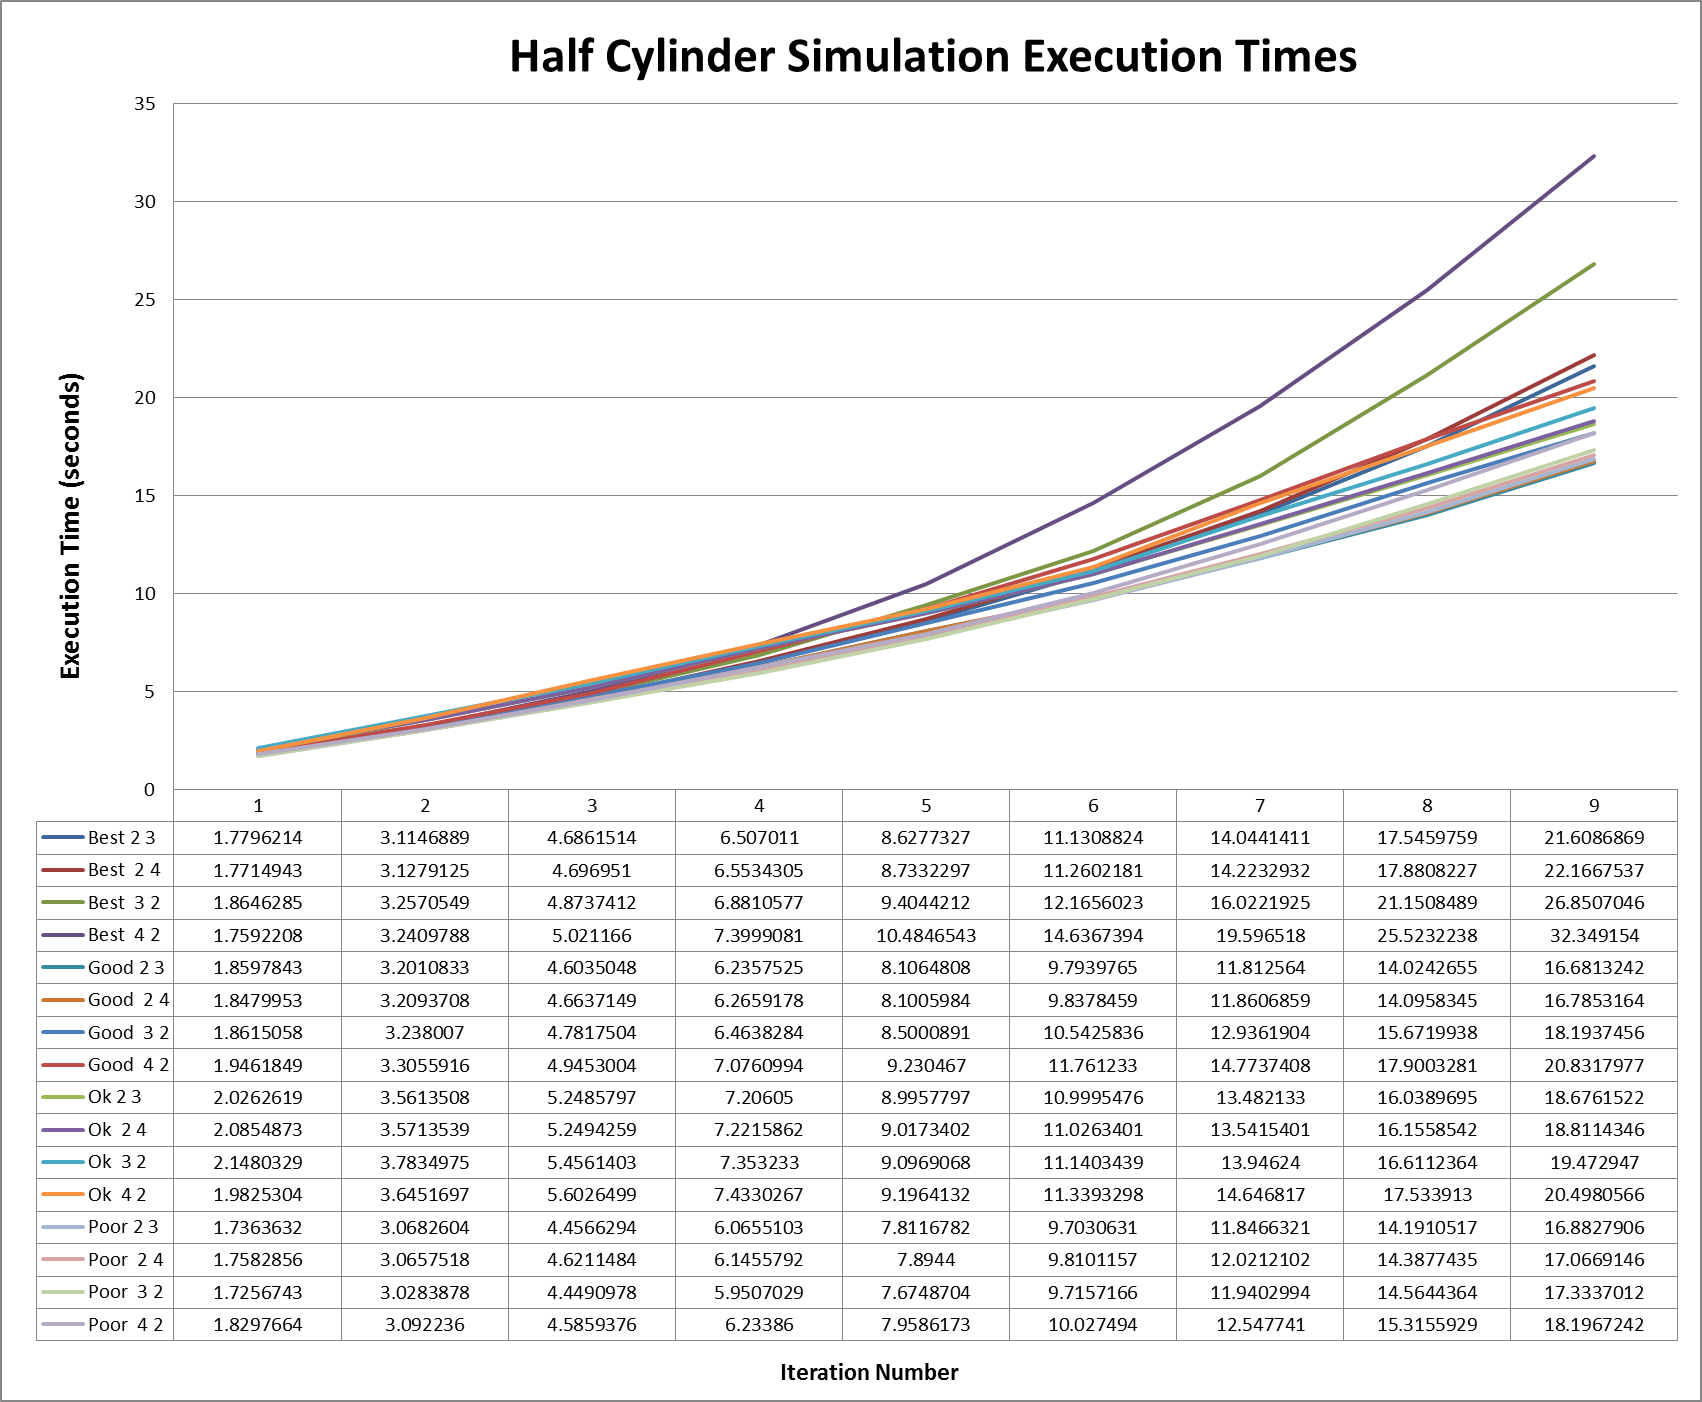
\includegraphics[width=120mm, scale=0.5]{../Graphics/HalfCylinder/ExecutionTimes.png}}
  \caption{Time taken per iteration using the different hybrid weightings with varying edge quality specifications}
\end{figure}

\newpage

\section{Gantt Chart for Project Time Management}
This appendix lists the main tasks that were undertaken for the project and how they fit into the time plan that was initially formulated at the start of the project.

\noindent
\textbf{Tasks:}

\begin{enumerate}[label=\Alph*]
\item Write supervisor project Proposal.
\item Review currently available FE tools that I can use as the basis for conducting my work.
\item Conduct research on current applications of AI and machine learning for FEA.
\item Given feasibility of work begin to build basic interfaces with FE tool and consider architecture for tool.
\item Conduct research on mesh assessment metrics allowing for automatic quality check of generated meshes.
- research metrics\\
- investigate building them into prototype of tool
\item Time allocation to catch up with University coursework.
\item Write interim report for dissertation (deadline 08 December).
\item Research possible methods for combining both stress based refinement and AI refinement\\
- explore research methods\\
- implement prototype of composition functions and run iteratively on basic model.
\item Take Christmas time off/revise other modules.
\item Research feasibility of distribution or concurrent execution of problem.
\item Develop/obtain a series of finite element models of increasing complexity to test current prototype on.
\item Having run the developed models look at fixing any problems that may have arisen as a result of increased complexity in geometry.
\item Analyse results from running prototype on range of models and analyse/cross reference results against those reported in papers.
\item Review and update methods before rerunning  them on the models to hopefully achieve improved results.
\item Begin to structure the layout/arguments I want to make for the final dissertation.
\item Write final dissertation (Deadline 6th April 2017).
\end{enumerate}
\pagestyle{empty}
\begin{landscape}


\begin{figure}[H]
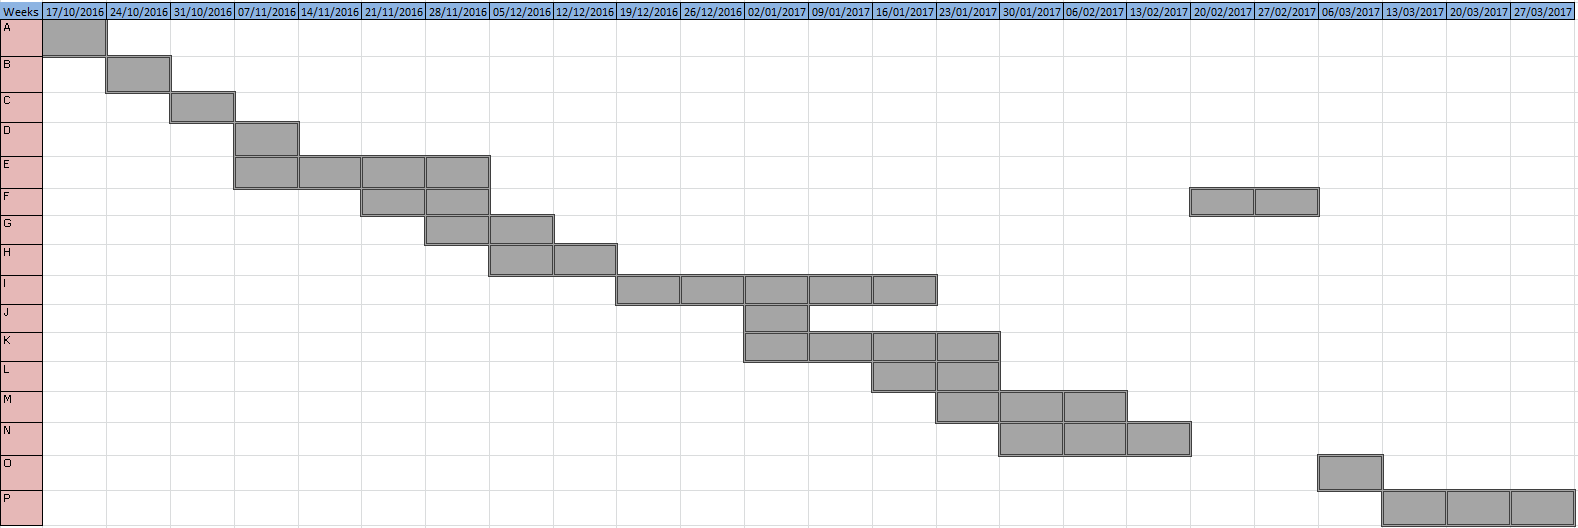
\includegraphics[width =630px, height=270px]{../Graphics/TimePlanUpdated2.png} \par
\caption{Gantt chart showing the initial plan for the projects progress}
\end{figure}
\end{landscape}

